\renewcommand{\chaptername}{Diseño de un puente H para el posicionador}
\graphicspath{{parte_4/puente_h/}}
\chapter{Diseño de un puente H para el posicionador} \label{cap:driver_motores}
\markright{Diseño de un puente H para el posicionador} 
\begin{center}
	\begin{tcolorbox}[colback=gray!5!white, %Color del fondo
		colframe=blue!75!black,
		title= \center{\Large{Resumen}} ]
		En esta sección, se diseña y seleccionan los componentes electrónicos para controlar los motores que mueven la antena. El circuito seleccionado es el denominado Puente H, el cual permite la inversión de polaridad para poder mover la antena en ambos sentidos. 
	\end{tcolorbox}
\end{center}    


\section{introducción}
	
	Se realiza el diseño y construcción de un puente H basado en transistores mosfet de canal P y canal N. Esto se realiza de esta manera porque se dispone de una única fuente de alimentación, y al usar estos dos tipos de transistores, no es necesario elevar la tensión respecto a la tensión de alimentación, para realizar el disparo de los mosfet. Los mosfet seleccionados son el IRFP240 (canal N) y el IRF 9530(canal P) ambos disponibles en el mercado local. Estos mosfet se han seleccionado por poder manejar las corrientes del motor que mueve la antena. En total se realizan dos puentes H, uno para cada motor y, por tanto, se muestra el análisis de uno solo de estos. Además, debe protegerse a cada puente H contra el cortocircuito debido a que los pines del microcontrolador se ponen en nivel bajo al cargar un código. Por tanto, se diseñan dos circuitos de control para el puente H, y luego se elige el diseño que se adapta a la hoja de datos de los transistores mosfet. Además, se hace un análisis térmico de los transistores mosfet, para que realicen una adecuada evacuación del calor.
	
	
\section{Análisis de los transistores Mosfet y BJT} 

Se analiza el funcionamiento de los transistores MOSFET y BJT cuando son usados como llave on/off. En general los MOSFET tienen rápida respuesta (del orden de nanosegundos), y soportan varios ampere de corriente. Estos, se utilizan para dirigir el sentido de giro de un motor, en una estructura conocida como puente H. Estos transistores Mosfet, son controlados por transistores BJT de propósito general. Cabe mencionar que esta selección se hizo de manera que estos transistores (MOSFET y BJT) puedan hallarse en el mercado local.   
%A continuación, se da una breve descripción de los transistores MOSFET y BJT, y en la sección siguiente, se muestran las características particulares de los dispositivos mosfet y BJT seleccionados.
%
\subsection{Transistor Mosfet} 

El transistor de tipo mosfet se basa en tres terminales, llamados Gate, Source y Drain. Existen de dos tipos: incrementales (o de enriquecimiento) y decrementales (o decrecimiento). El mosfet de tipo decremental no se utiliza, y por tanto, solamente se hace mención de él y no se darán detalles de su funcionamiento. El tipo de mosfet utilizado es el incremental. 


El mosfet incremental (válido para el decremental también), se denominan de canal N o de Canal P. Se brinda la explicación sobre el mosfet de canal N, y el de canal P, se deben invertir las polaridades de tensión. En el mosfet de canal N, se basa que al existir una tensión entre Gate y Source positiva, más alta que una tensión denominada ``tensión umbral''($V_{t}$) el dispositivo mosfet, empieza a conducir, en una zona de operación llamada de saturación. El diagrama de un mosfet es el que muestra la figura \ref{fig:mosfet_str_model}. No se dan las explicaciones sobre la física del dispositivo de estado sólido, pero se ilustra a continuación en conjunto con el circuito de prueba: 

\begin{figure}[ht!]
	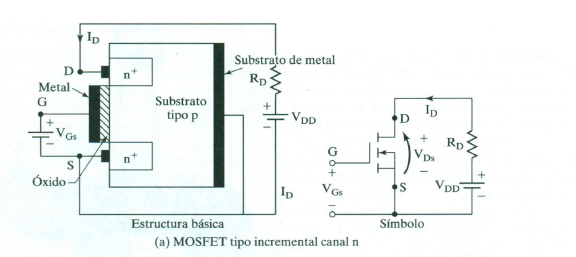
\includegraphics{mosfet_estr}
	\caption{Esquema de un mosfet a la izquierda. A la derecha se muestra el modelo circuital y su símbolo}
	\label{fig:mosfet_str_model}
\end{figure}

Si se realiza el circuito de la derecha sobre un mosfet de canal N, se obtienen las siguientes curvas:

\begin{figure}[ht]
	\begin{subfigure}{0.5\linewidth}
		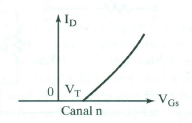
\includegraphics[width=\linewidth]{curva_1_mosf}
		\caption{Gráfica $V_{gs}$ vs $ I_d$}
	\end{subfigure}
	\hfil
	\begin{subfigure}{0.5\linewidth}
		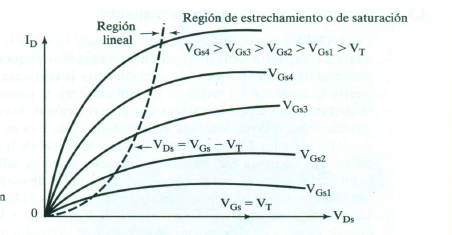
\includegraphics[scale=0.75]{curva_2_mosf}
		\caption{Gráfica $V_{ds}$ vs $ I_d$ con $V_{gs}$ constante}
		\label{fig:vds_vs_id_mosfetop}	
	\end{subfigure}
\caption{Curvas características de un transistor mosfet de canal N}
\end{figure}

Donde $V_t$ es la tensión umbral del dispositivo. Se observa en la curva \ref{fig:vds_vs_id_mosfetop} que existen tres regiones de operación del mosfet, estas son:
\begin{enumerate}
	\item Región de corte: ocurre cuando $V_{gs}<V_t$. En esta condición la corriente entre Drain y Source es nula, es decir, se tiene una llave abierta.
	\item  Región de saturación: en esta zona se cumple la siguiente desigualdad: $V_{gs}>V_t$ y $V_{gs}-V_{t}<V_{ds}$. En esta zona se tiene la saturación y la llave se comporta como una fuente de corriente controlada por tensión. 
	\item Región óhmica o zona óhmica: en este caso se tiene la siguiente desigualdad: $V_{gs}>V_t$ y $V_{gs}-V_t>V_{ds}$
\end{enumerate} 

En la zona óhmica, se presenta una resistencia, llamada $R_{ds}$, que es cuando empieza a conducir el mosfet. Este valor viene dado por la pendiente de la recta en la zona óhmica. Es decir la siguiente relación: 
\begin{equation*}
	R_{ds} =\frac {V_{gs}}{I_{ds}} 
\end{equation*}

Se utiliza la zona óhmica, debido a que la corriente que circula por la carga es variable, y se debe fijar la tensión entre Gate y Source. Por este motivo, el trabajo y diseño del puente H, se realiza en esta zona. 

\subsection{Transistor BJT como llave electrónica}

El transistor BJT es un transistor que tiene tres junturas, de tipo NPN y PNP. Este dispositivo puede utilizarse como llave electrónica o para la amplificación de señales (zona activa). Para este trabajo, lo utilizamos como llave, y se explicara su funcionamiento en esta zona, dejando de lado la zona activa de los transistores. El símbolo del transistor es el siguiente: 
\vspace{-5mm}
\begin{figure}[h]
	\begin{subfigure}{0.5\textwidth}
		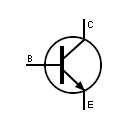
\includegraphics{simbol_npn}
		\caption{símbolo del transistor BJT de tipo NPN }
	\end{subfigure}
	\hfill 
	\begin{subfigure}[h]{0.5\textwidth}
		
\includegraphics{simbol_pnp}
		\caption{símbolo del transistor BJT de tipo PNP }
	\end{subfigure} 
\caption{Símbologia electrica de transistores BJT} 
\end{figure}
\vspace{-5mm}

En la figura anterior, se ven los dos tipos de transistores NPN y PNP. En ella se observa que es un dispositivo de tres terminales, denominados emisor(E) – base(B) y colector (C) respectivamente.  

Dado que tiene tres terminales, podemos asociarlas a un tipo de juntura NP o PN, y en base a la polarización de estas, determina el uso del transistor. Estas junturas son Colector – Base y Base Emisor. En el caso de un transistor NPN, la juntura Colector Base es de tipo NP, y la juntura Base – emisor es de tipo PN. 

En este tópico, cabe decir, que el transistor PNP o NPN, poseen distintas configuraciones según sean los circuitos de configuración (topología del circuito): emisor común – base común y colector común. En este apartado, solo se considera la topología emisor común, ya que es aquella que mayoritariamente usa al transistor como llave on/off.  

Los transistores BJT, ya sean PNP o NPN, tienen un conjunto de curvas características, que determinan como es la transferencia entre los parámetros del transistor. Estas curvas, se muestran en la figura \ref{fig:curvas_bjt} para el transistor de tipo NPN. Si desea las curvas del transistor PNP, basta con invertir las tensiones: 

\begin{figure}[h!]
	%\centering 
	\begin{subfigure}{0.4\linewidth}
		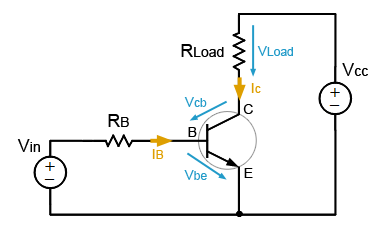
\includegraphics[scale=0.5]{curva_entrada_bjt}
		\caption{Curva característica de entrada}
		\label {fig:circ_pol_bjt}
	\end{subfigure}
	\begin{subfigure}{0.4\linewidth}
		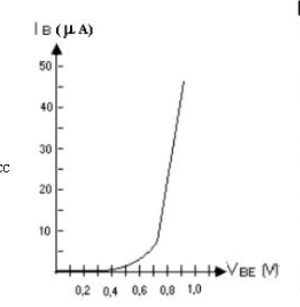
\includegraphics[scale=0.5]{curva_entrada_bjt_1}
		\caption{Circuito característico en topologia emisor común para obtener las curvas características}
		\label{fig:ib_vs_vbe}
	\end{subfigure}
	\hspace{50cm}
	\begin{subfigure}{0.4\linewidth}
		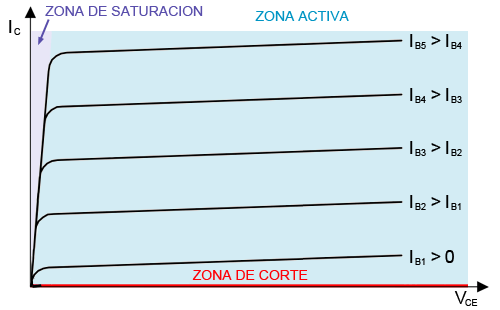
\includegraphics[scale=0.5]{Curva_ic_vs_vce}
		\caption{Curva característica regiones de operación de un transistor}
		
		\label{fig:Ic_vs_vce}
	\end{subfigure}
\caption{Curvas características de un transistor BJT}
\label{fig:curvas_bjt}
\end{figure}

Se observa en la figura \ref{fig:ib_vs_vbe} que la relación entre la corriente de base y la tensión base emisor (que es una juntura pn en este caso), se comporta como si fuese un diodo.  En la figura \ref{fig:Ic_vs_vce} se observa que el transistor tiene tres regiones de operación: saturación – activa y corte. La zona de corte, se da cuando la corriente de base es nula. En la región activa, la corriente de colector es proporcional a la corriente de base. Este factor de proporción se denomina ``ganancia del transistor'', y se lo denota con $\beta$ o con $h_{FE}$, y son un parámetro individual de cada transistor. En otras palabras, en la zona activa se cumple: 
\begin{equation} \label{eq:bjt_zona_act}
	I_c = \beta I_b
\end{equation}

En la zona de saturación, se observa (ver figura \ref{fig:Ic_vs_vce}) que la relación no se cumple, es más, se observa que la relación entre la corriente de base a colector es mayor que la de colector entre la ganancia del transistor. En otras palabras, se cumple que: 	

\begin{equation}
	I_b > \frac{I_c}{\beta} 
\end{equation}

Cabe destacar, que esto ocurre por la polarización de la juntura. En el caso de corte, ambas junturas se polarizan en inversa, y en saturación, ambas se polarizan en directa. En este estado, la tensión $V_{ce}$ de la figura \ref{fig:circ_pol_bjt} es muy pequeña, polarizando entre colector y base de forma directa. Si la juntura Base emisor se polariza en polarización directa, mientras la juntura entre colector y base en polarización inversa, se está en zona activa (es decir, en la zona de amplificación y se cumple la ecuación \ref{eq:bjt_zona_act}). 


Por las gráficas de la figura \ref{fig:curvas_bjt},se observa que la zona de trabajo de un transistor depende fuertemente de la corriente de base, y la topología de circuito que se esté utilizando. Por ello, es que es necesario, determinar dos parámetros importante: Resistencia de base($R_B$ en la figura \ref{fig:circ_pol_bjt}) y máxima corriente de colector en zona activa Este parámetro, permite determinar si el transistor se satura o no, pues es necesario elevar la corriente de base por encima de una valor mínimo para que el transistor entre en saturación.  
Para calcular la resistencia de base, se analiza el circuito que está a continuación: 


\begin{figure}[ht!]
	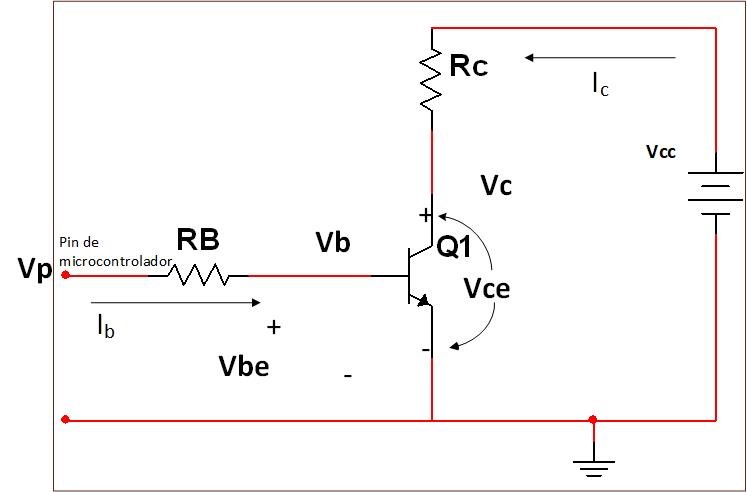
\includegraphics[scale=0.8]{circuito_analisisBJT} 
	\caption{Circuito para el cálculo de la resistencia de base de un transistor bipolar NPN. En este diagrama donde dice ``pin de microcontrolador'' es el control del transistor entre corte y saturación realizado mediante la programación del sistema embebido}
	\label{fig:calc_RB}
\end{figure}


De la figura \ref{fig:calc_RB}, donde dice ``pin del microcontrolador'', es el pin destinado a poner en corte al transistor, o saturarlo. Dada una resistencia de colector ($R_c$ en figura \ref{fig:calc_RB}), y una tensión de entrada $V_p$ (ver figura \ref{fig:calc_RB}), se van obtienen las ecuaciones para el cálculo de $R_b$. 
Si realizamos la malla entre colector y emisor, cerrándola sobre el mismo transistor, se tiene la siguiente ecuación de Kirchhoff: 

\begin{equation} \label{eq:state_bjt}
	V_{CE} = V_{BE} + V_{CB} \rightarrow V_{CB}= V_{CE} - V_{BE}
\end{equation}

Para que el transistor se encuentre en estado de corte, se debe cumplir que $V_{CB}>0$  y la tensión entre $V_{BE}<0$ o menor a un valor que especifique el fabricante del dispositivo (generalmente 0.6V), la saturación se da cuando $V_{BE}>0$ y $V_{CB}<0$. Si un transistor cumple que $V_{CB}>0$ y $V_{BE}>0$, se puede afirmar (en base a la expresión \ref{eq:state_bjt}) $V_{CE}>V_{BE}$, y el transistor esta en zona activa.

Si suponemos el transistor en zona activa, de la expresión \ref{eq:state_bjt}, la corriente máxima de colector, la podemos obtener, igualando $V_{CB}=0$. Si esto ocurre, $I_C$  adopta el valor de (resolviendo la malla de la derecha de la figura \ref{fig:calc_RB}):
\begin{equation} \label{eq:ICmaxSat}
	I_{Cmax} = \frac{V_{CC} - V_{CE}}{R_c} = \frac{V_{CC} - V_{BE}}{R_c}
\end{equation} 

y el valor de la corriente de base para esta condición es: 
\begin{equation}
	I_{Bmin} = \frac{I_{Cmax}}{\beta}
\end{equation}

Luego, si la corriente por la base, aumenta por encima de $I_{Bmin}$ , entonces $V_{BE} $ aumenta la corriente de colector, disminuyendo $V_{CE}$   y esta baja hasta un valor menor a $V_{BE}$. En este punto, la tensión ala cual la tensión de $V_{CE}$ se denomina tensión colector-emisor de saturación, y la denotamos: $V_{CE(sat)}$. Para obtener la corriente de colector en estas condiciones: 
\begin{equation}
	I_{Csat} = \frac{V_{CC}- V_{CEsat}}{R_c} 
\end{equation}

Por tanto, dado una $I_{Bmin}$, la $I_{B}$ que circule por la base, debe ser mayor a esta $I_{Bmin}$. Con estos datos, podemos hallar una Resistencia de base, que satisfaga estos requerimientos. De la figura \ref{fig:calc_RB}, usando la malla del lado izquierdo:
se obtiene que\footnote{Para llegar a esta expresión, se debe plantear que $I_{b}>I_{bmin}$ y despejar $R_b$}: 
\begin{equation} \label{eq:select_rb}
	R_B < \frac{V_p-V_{BE}}{I_{bmin}}
\end{equation} 

Luego, se debe seleccionar una $R_B$ que satisfaga la desigualdad \ref{eq:select_rb}.  
Cuando la tension $V_p$ es cero, el transistor está cortado, y no hay circulación de corriente en la malla. En esta situación, ocurre que $V_{BE}=0$. Por ende, el procedimiento para seleccionar la resistencia, tanto de colector, como de base, se basa en las corrientes de base y colector. Estas, tienen valores máximos y mínimos brindados por los fabricantes, y se debe tener la hoja de datos al seleccionar esta resistencia. 

\subsection{Componentes seleccionados} 


Los mosfet se eligien de tal manera que cumplan tres requerimientos:
\begin{itemize}
	\item Disponibilidad en el mercado local 
	\item Menor resistencia entre Drain y source 
	\item Soporten una corriente variable entre 0.4 A y 7 A   
	
\end{itemize}
 
Los mosfet que se encuentran en el mercado local que cumplen todos los requisitos son el IRFP240(canal N) y el IRF9530(canal P). Una vez seleccionados, resta elegir la tensión entre gate y source para ambos dispositivos. Además, se eligieron dos de canal P y dos de canal N ya que se cuenta con una única fuente de tensión. 


\subsubsection{Mosfet IRFP240} 

Este mosfet es de canal N, con una $R_{ds}$ máxima de 0.18 ohm. Su tensión umbral $V_{t}$ oscila entre 2V y 4V. Por tanto, la tensión entre $V_{gs}$ debe ser superior a 4 volts para asegurar su conducción. Para decidir qué tensión se debe aplicar entre Gate y Source, se debe tener en cuenta, la tensión máxima que soporta entre $V_{gs}$. Este dato, extraído de la hoja de datos es 20V. De la discusión precedente, obtenemos que Vgs debe estar comprendida entre 4v y 20v (ver \cite{IRFP240}). 
Debido a que la tensión entre gate y source está definida sobre un rango de tensiones, se debe elegir aquella que minimice la tensión entre Drain y source, y tenga un rango de operación completo entre 5 Ampere y 0.44 Ampere (corriente consumida por el motor). La curva $I_d$ a $V_{gs}$ a una temperatura de 25° C se obtiene del datasheet, y se muestra en la figura \ref{fig:irfp_240_id_vs_vds}: 

\begin{figure}[ht!]
	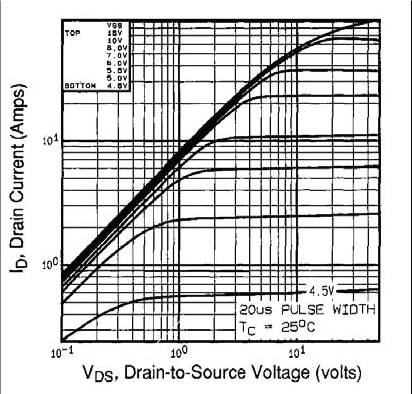
\includegraphics{curva_datasheet_1} 
	\caption{Diagrama de Id vs Vgs del mosfet IRFP240. Esta curva la brinda el fabricante, para distintos valores de Vgs}
	\label{fig:irfp_240_id_vs_vds}
\end{figure}

De la figura anterior(\ref{fig:irfp_240_id_vs_vds}) se observa que la tensión $V_{gs}$ más chica es de 4.5 V, y se obtiene una corriente máxima de aproximadamente 0.5 Ampere. La curva siguiente, se tiene $V_{gs}$ de 5V, y una corriente máxima de 2.3 Ampere aproximadamente. La que sigue, tiene una tensión de 5.5 V y una corriente de 6 ampere, y luego sigue aumentando $V_{gs}$ y se observan las distintas tensiones entre Drain y source. La corriente que maneja nuestra carga oscila entre 0.44 Ampere y 4 Ampere. De la gráfica, observamos que el menor $V_{gs}$ que encontramos es 7 Volts, y se obtiene un $V_{gs}$ que oscila entre 0.1Volt y 0.7volts aproximadamente (datos extraídos del gráfico). 

Por el hecho de que el valor dentro del gráfico es aproximado, se realiza, una simulación del dispositivo, con el software NI Multisim. El circuito para simular es el que se muestra en la figura \ref{fig:mosfet_str_model}, con una tensión de $V_{gd}$ entre 6.5 Volts y 7.5Volts, con iteraciones cada 0.3V y $V_{ds}$ oscilando entre 0volts y 24 volts. El resultado se muestra a continuación:

\begin{figure}[ht!]
	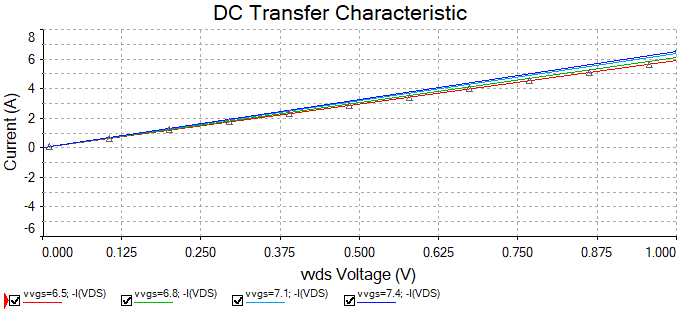
\includegraphics[width=\linewidth,height=5cm]{simul_irfp240} 
	\caption{Resultados de simulación del mosfet IRFP240. En él, se fija $V_{gs}$, y se hace variar $V_{ds}$, y luego se grafica la corriente en función de $V_{ds}$}
	\label{fig:simul_irfp240}
\end{figure}

Los resultados mostrados en la figura \ref{fig:simul_irfp240}, para la corriente que se requiere, los valores de caída de tensión entre Drain y source sobre el mosfet oscilan entre 0.1 Volt y 0.625 Volts (resultado de la simulación). Del grafico (figura \ref{fig:simul_irfp240}) se observa, que una tensión $V_{gs}$ superior a 7 volts, se tiene la misma resistencia aproximadamente, dentro del rango de operación del motor. 










%
%\begin{table}[h]
%%	\hspace{-30mm}
%\resizebox{\linewidth}{!}
%{
% \begin{threeparttable}
%	\begin{tabular}{|c|c|c|c|c|c|c|c|c|c|c|c|} 
%%--- fila con titulos de tabla  -----------------------% 
%		 \hline
%		 \multicolumn{5}{|c|}{ \multirow{2}{20mm}{parámetros circuitales}} & 
%		 \multicolumn{3}{c|}{estado} & 
%		 \multicolumn{2}{c|}{\multirow{2}{20mm}{Condiciones de corte}} & 
%		 \multirow{2}{20mm}{Condiciones de sat} 
%		 & \multirow{3}{20mm}{cumple req} \\ \cline{6-8}
%%---- segunda fila ---- 
%		 \multicolumn{5}{|c|}{} &  \multicolumn{2}{c|}{corte} & saturación & \multicolumn{2}{c|}{} && \\ \cline{1-11}
%% -----------------------variables -----------------------%		 
%		 $I_s$[ma]&$R_1$[K$\Omega$]&$R_2$[K$\Omega$]&$I_c$[ma]&$R_3$[K$\Omega$] & $V_{g1}$[V]& $V_{g4}$[V]& $V_{g1}$[V] & $V_{g1}>22V$ & $V_{g4}>7v$ & $V_{g1}<9V$ & \\ \hline 
%%----------------- datos ----------------------------------% 
%	1 & 16&9&0.1 &216&22.5 &6.96 &21.89 &\checkmark & \xmark  & \xmark & no \\ \hline
%	2 & 8 & 4 & 0.2 & 108 & 22.4 & 21.6 & 16 & \checkmark & \checkmark & \xmark & no \\ \hline   	
%	5 & 3.1 & 1.7 & 0.5 & 43.2 & 22.45 & 21.6 & 8.5 & \checkmark & \checkmark	& \checkmark &Sí\tnote{1} \\ \hline 
%	3 & 6 & 2 & 0.3 & 72 & 22.2 & 21.6 & 6 & \checkmark & \checkmark & \checkmark & si\tnote{1}   \\ \hline
%	10 & 2 & 0.4 & 0.8 & 27.6 & 22.4 & 22.08 & 4 & \checkmark & \checkmark & \checkmark & si \tnote{1} \\ \hline 
%	\end{tabular}
%	\begin{tablenotes}
%		\small
%		\item[1] En este caso, se cumplen las condiciones para su uso, solo que el transistor mosfet elegido soporta una tension máxima de 20 volts entre Gate y Source. 
%	\end{tablenotes}
%	\end{threeparttable}
%}
%\caption{Valores que se obtienen mediante el proceso de iteración}
%\end{table}	
%

%
%\begin{table}[h]
%	%	\hspace{-30mm}
%	\resizebox{\linewidth}{!}
%	{
%		\begin{threeparttable}
%			\begin{tabular}{|c|c|c|c|c|c|c|c|c|c|c|c|} 
%				%--- fila con titulos de tabla  -----------------------% 
%				\hline
%				\multicolumn{5}{|c|}{ \multirow{2}{20mm}{parámetros circuitales}} & 
%				\multicolumn{3}{c|}{estado} & 
%				\multicolumn{2}{c|}{\multirow{2}{20mm}{Condiciones de corte}} & 
%				\multirow{2}{20mm}{Condiciones de sat} 
%				& \multirow{3}{20mm}{cumple req} \\ %\cline{6-8}
%				%---- segunda fila ---- 
%				\multicolumn{5}{|c|}{} &  \multicolumn{2}{c|}{corte} & saturación & \multicolumn{2}{c|}{} && \\ \cline{1-11}
%				% -----------------------variables -----------------------%		 
%				$I_s$[ma]&$R_1$[K$\Omega$]&$R_2$[K$\Omega$]&$I_c$[ma]&$R_3$[K$\Omega$] & $V_{g1}$[V]& $V_{g4}$[V]& $V_{g1}$[V] & $V_{g1}>22V$ & $V_{g4}>7v$ & $V_{g1}<9V$ & \\ \hline 
%				%----------------- datos ----------------------------------% 
%	
%	\end{tabular}
%	\begin{tablenotes}
%	\small
%	\item[1] En este caso, se cumplen las condiciones para poder usarlo, solo que la limitante es el dispositivo mosfet elegido, ya que su tensión máxima que soporta entre Gate y Source es 20 volts. 
%	\end{tablenotes}
%	\end{threeparttable}
%}
%\caption{Valores que se obtienen mediante el proceso de iteración}
%\end{table}	
